\documentclass{standalone}
\usepackage{tikz,tikz-3dplot}
\usepackage{tikzscale}
\usepackage{csvsimple}
\usepackage{bm}
\usepackage{pgfplots}
\usepackage{xcolor}
\pgfplotsset{compat=newest}

% MATLAB colors (lines)
\definecolor{c1}{rgb}{0, 0.4470, 0.7410} % blue
\definecolor{c2}{rgb}{0.8500, 0.3250, 0.0980} % orange
\definecolor{c3}{rgb}{0.9290, 0.6940, 0.1250} % yellow
\definecolor{c4}{rgb}{0.4940, 0.1840, 0.5560} % purple
\definecolor{c5}{rgb}{0.4660, 0.6740, 0.1880} % green
\definecolor{c6}{rgb}{0.3010, 0.7450, 0.9330} % light blue
\definecolor{c7}{rgb}{0.6350, 0.0780, 0.1840} % red

\begin{document}

% 2d plot
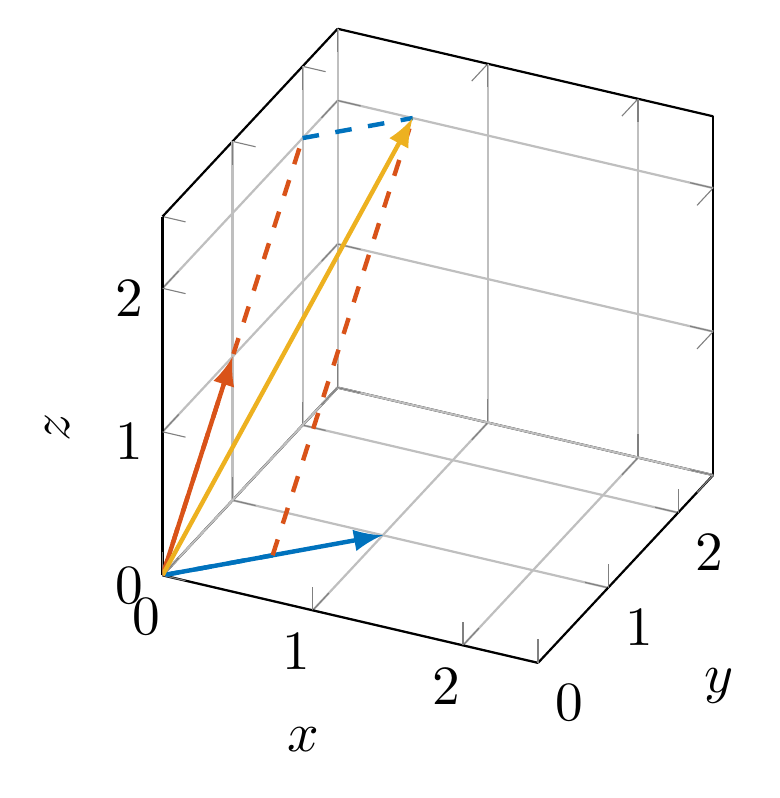
\begin{tikzpicture}[scale=2]
    \begin{axis}[
            xlabel=$ x $, ylabel=$ y $, zlabel=$ z $,
            xmin=0, xmax=2.5,
            ymin=0, ymax=2.5,
            zmin=0, zmax=2.5,
            grid, axis equal image,
        ]
        \addplot3[-latex, c1, thick] coordinates {(0,0,0) (1,1,0)};
        \addplot3[dashed, c1, thick] coordinates {(0,0,0) (0.5,0.5,0)};

        \addplot3[-latex, c2, thick] coordinates {(0,0,0) (0,1,1)};
        \addplot3[dashed, c2, thick] coordinates {(0,0,0) (0,2,2)};

        \addplot3[c1, thick, dashed] coordinates {(0,2,2) (0.5,2.5,2)};
        \addplot3[c2, thick, dashed] coordinates {(0.5,0.5,0) (0.5,2.5,2)};

        \addplot3[-latex, c3, thick] coordinates {(0,0,0) (0.5,2.5,2)};
    \end{axis}
\end{tikzpicture}

\end{document}